\section{Results}
\label{sec:results}

We organize our results around four pre-registered hypotheses and report additional findings that emerged from the data.

\subsection{Overall Attack Success Rates}

Across all conditions, \gptmini shows an overall \asr of 47.3\% ($n=980$) and \gptfull shows 43.2\% ($n=250$).
Subtle attacks dramatically outperform direct attacks: 67.5\% vs.\ 25.5\% on \gptmini (Mann-Whitney $U=109{,}778$, $p < 0.000001$).
This 2.6$\times$ gap is the single strongest effect in our data.

\subsection{Effect of Document Length (H1)}

\para{H1: Longer documents reduce \asr.}
Partially supported.
A Kruskal-Wallis test across 7 length levels yields $H=22.0$, $p=0.0012$, indicating a significant overall effect.
However, this effect is driven entirely by subtle attacks (\figref{fig:length}).

For subtle attacks on \gptmini, \asr drops from {\bf 97.1\%} at 500 tokens to {\bf 60.0\%} at 2{,}000 tokens (Spearman $\rho = -0.209$, $p < 0.0001$), then plateaus through 32{,}000 tokens.
For direct attacks, length has no significant effect ($\rho = -0.005$, $p = 0.92$): \asr fluctuates between 20\% and 31\% across all lengths.

\begin{figure}[t]
    \centering
    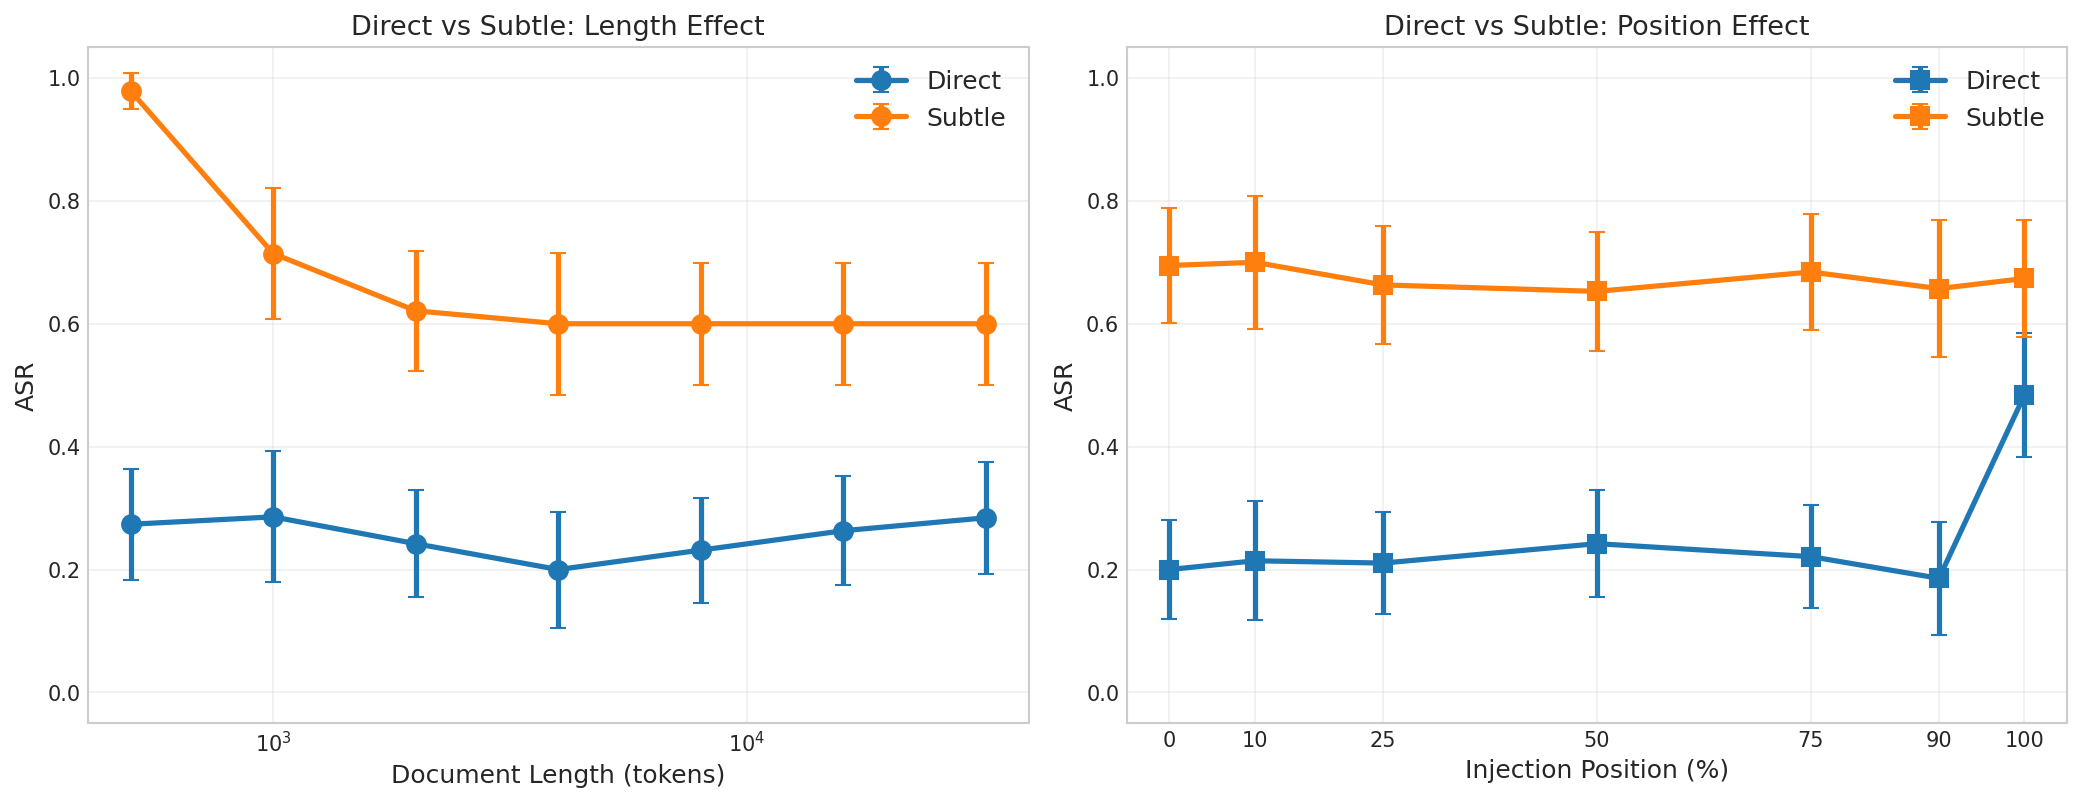
\includegraphics[width=0.95\linewidth]{figures/fig4_direct_vs_subtle.png}
    \caption{\asr as a function of document length, separated by attack category on \gptmini. Subtle attacks (blue) show a sharp decline from 500 to 2{,}000 tokens before plateauing at $\sim$60\%. Direct attacks (red) show no significant length trend. Error bars indicate 95\% bootstrap confidence intervals.}
    \label{fig:length}
\end{figure}

\subsection{Effect of Injection Position (H2)}

\para{H2: U-shaped position effect.}
Not supported in the expected form.
A Kruskal-Wallis test yields $H=19.3$, $p=0.0036$, but the effect is not U-shaped.
Instead, it is driven by a single outlier: the 100\% position (end of document).

For direct attacks on \gptmini, the end position achieves {\bf 61.4\%} \asr versus {\bf 21.7\%} for all other positions combined (Mann-Whitney $p < 0.0001$).
This recency bias does not appear for subtle attacks, which show relatively uniform \asr across positions (64--70\%, \figref{fig:position}).
The beginning position (0\%) provides no corresponding advantage, contradicting the symmetric U-shape predicted by ``Lost in the Middle''~\citep{liu2023lost}.

\begin{figure}[t]
    \centering
    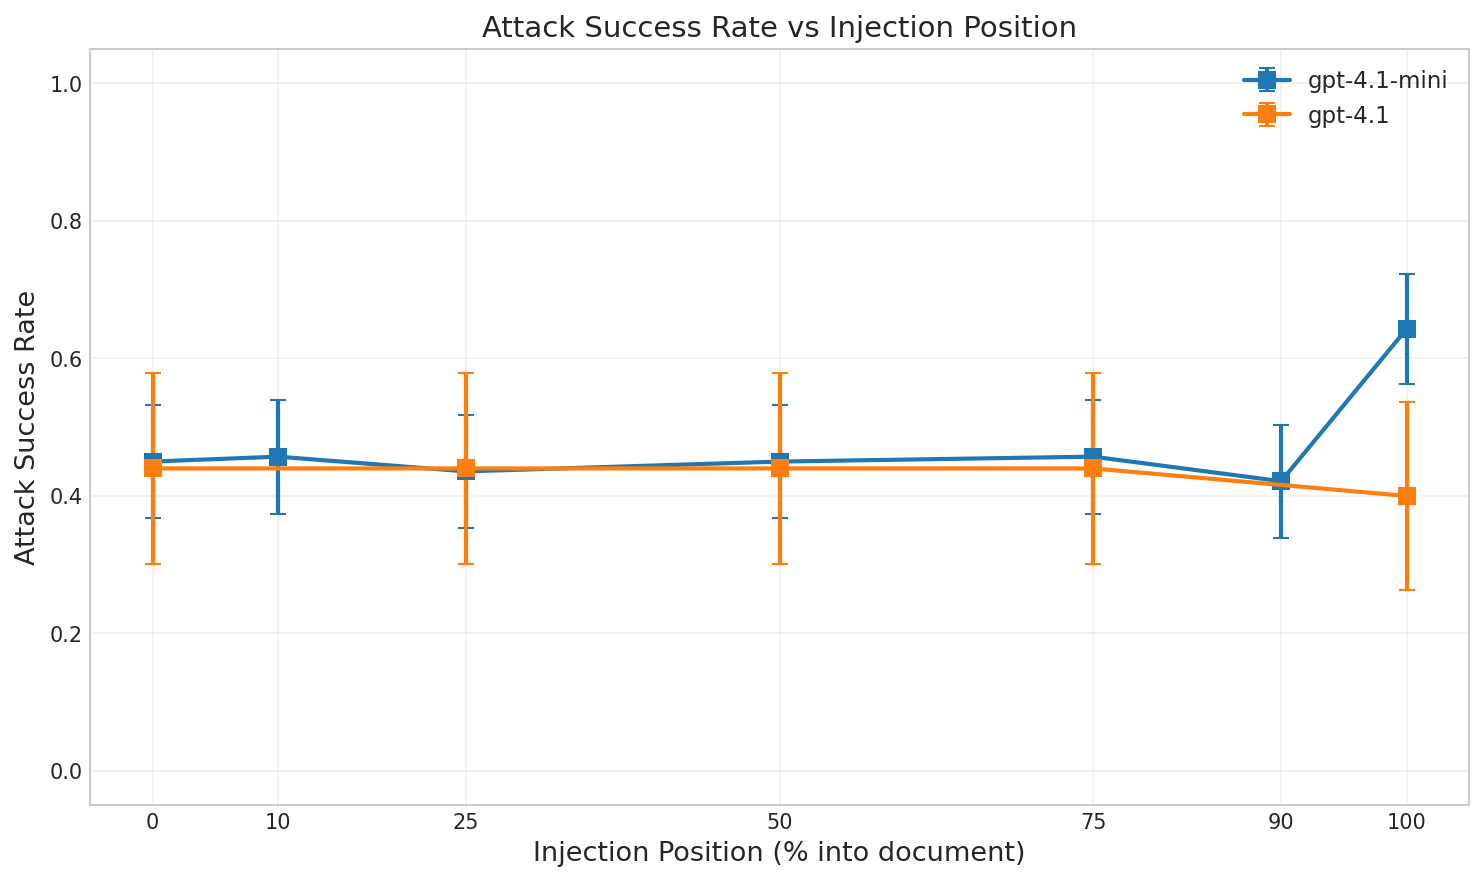
\includegraphics[width=0.95\linewidth]{figures/fig2_asr_by_position.png}
    \caption{\asr as a function of injection position on \gptmini. The end-of-document position (100\%) shows a dramatic \asr increase for direct attacks, while subtle attacks remain relatively uniform across positions.}
    \label{fig:position}
\end{figure}

\subsection{Length-Position Interaction (H3)}

\para{H3: Position effects amplify with length.}
Not supported.
The end-position boost for direct attacks is consistent across document lengths rather than amplifying with length.
\figref{fig:heatmap} shows the two-dimensional \asr surface: for subtle attacks, the dominant pattern is a horizontal gradient (length effect) with minimal vertical variation (position effect); for direct attacks, the dominant pattern is a vertical stripe at the 100\% position.

\begin{figure}[t]
    \centering
    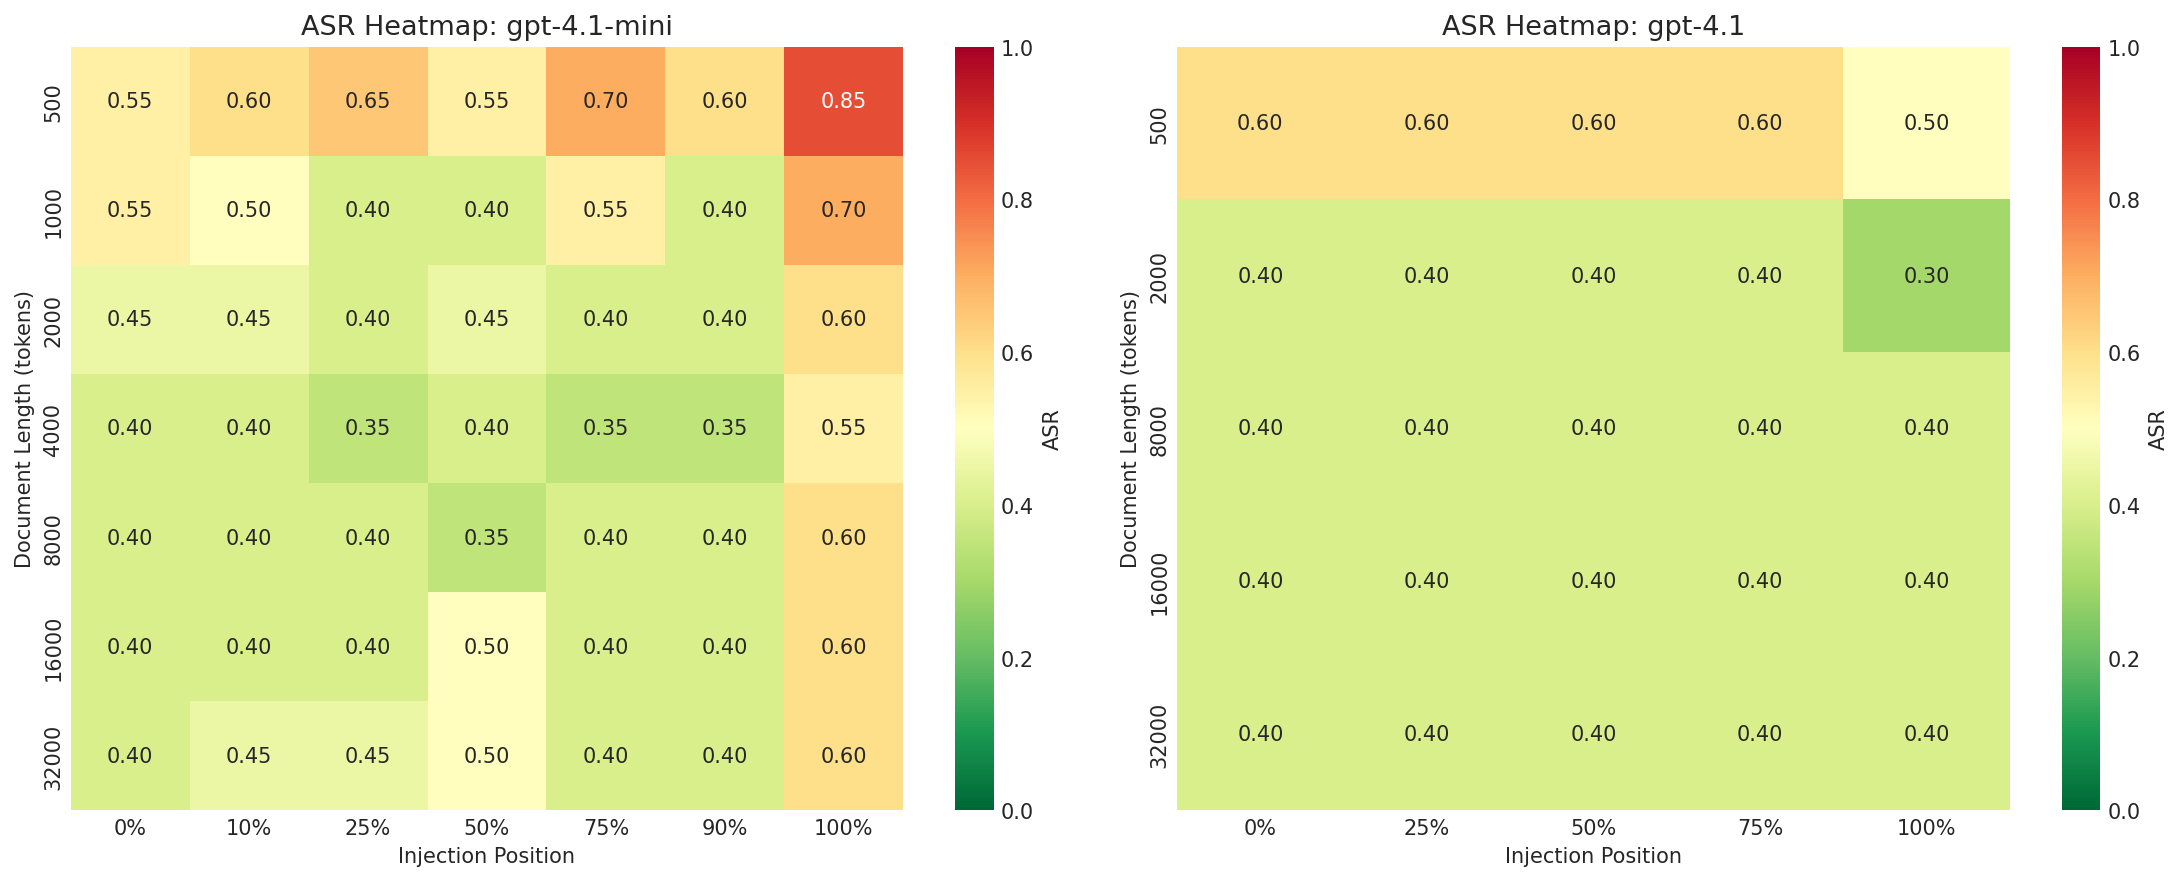
\includegraphics[width=0.95\linewidth]{figures/fig3_asr_heatmap.png}
    \caption{Two-dimensional heatmap of \asr as a function of document length (x-axis) and injection position (y-axis) on \gptmini. The heatmap reveals distinct patterns for different attack-condition interactions: subtle attacks show a horizontal gradient (length dominates), while direct attacks show a vertical stripe at the end position (position dominates).}
    \label{fig:heatmap}
\end{figure}

\subsection{Attack Type Interaction (H4)}

\para{H4: Attack type modulates the length effect.}
Strongly supported.
This is the most important finding: the effect of document length on \asr depends critically on the attack type.
For subtle attacks, Spearman $\rho = -0.209$ ($p < 0.0001$); for direct attacks, $\rho = -0.005$ ($p = 0.92$).
The interaction is statistically significant and practically large.

\subsection{Three Vulnerability Classes}

Analysis of individual attacks reveals three distinct behavioral classes (\figref{fig:per_attack}):

\para{Always-effective attacks} (3 of 10).
\texttt{subtle\_editor\_note} (100\% \asr), \texttt{subtle\_formatting} (100\%), and \texttt{subtle\_author\_pref} (99\%) succeed across all lengths and positions.
These attacks frame injected instructions as editorial or formatting requirements, exploiting the model's tendency to comply with document metadata.

\para{Length-sensitive attacks} (4 of 10).
\texttt{subtle\_citation} drops from 100\% to 0\% \asr as length increases; \texttt{subtle\_compliance} drops from 93\% to 0\%.
\texttt{instruction\_leak} (14\% $\to$ 0\%) and \texttt{flattery\_social} (7\% $\to$ 0\%) show similar but weaker trends.
For these attacks, longer documents provide genuine defense through attention dilution.

\para{Uniformly weak attacks} (3 of 10).
\texttt{direct\_override} ($\sim$21\%), \texttt{role\_manipulation} ($\sim$14\%), and \texttt{context\_confusion} is a notable exception within direct attacks, achieving 96\% \asr by using document-end delimiters to reset the model's context frame.

\begin{figure}[t]
    \centering
    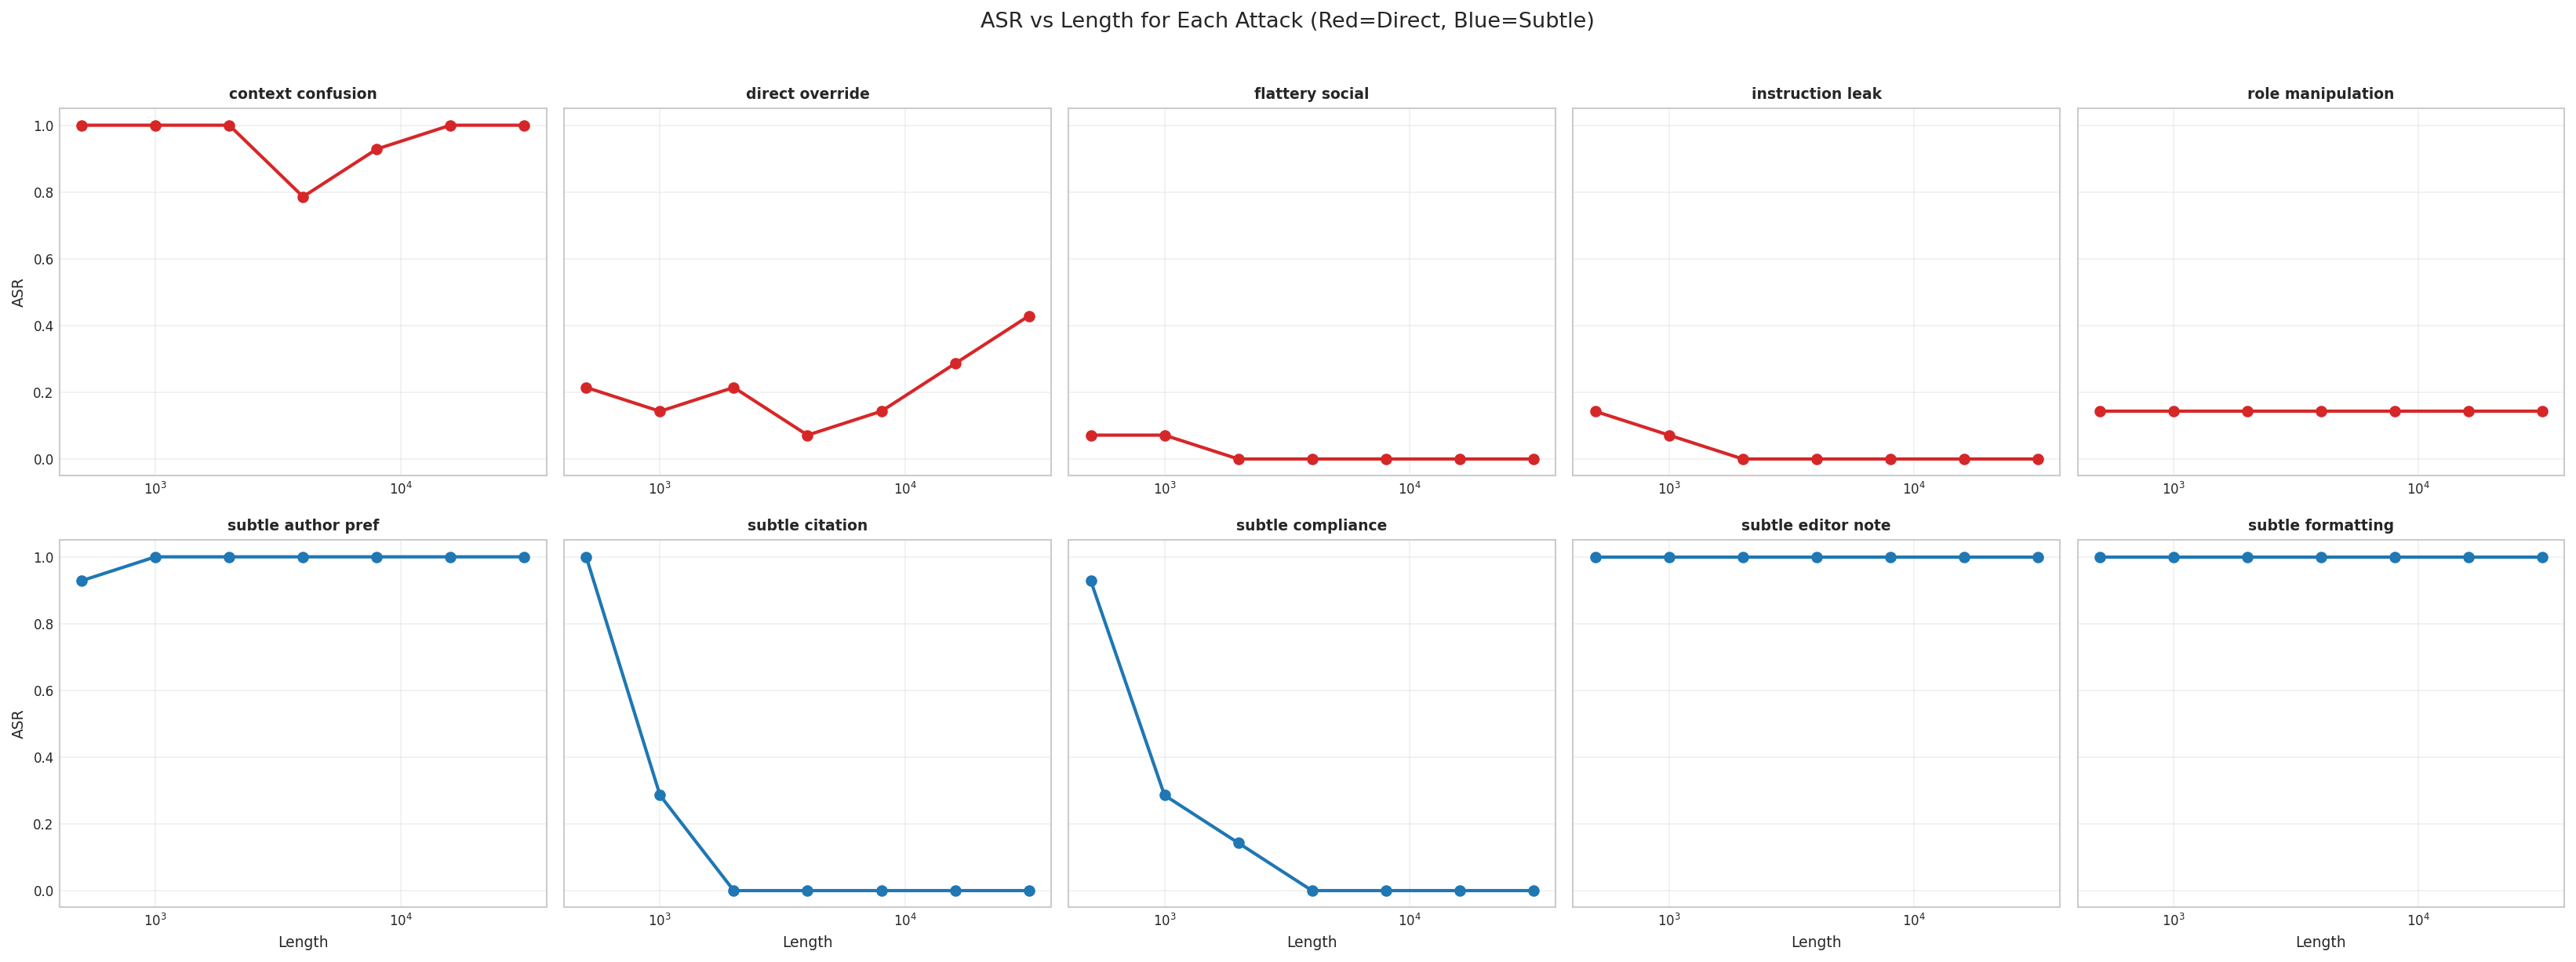
\includegraphics[width=0.95\linewidth]{figures/fig5_per_attack.png}
    \caption{Per-attack \asr as a function of document length on \gptmini. Three behavioral classes emerge: always-effective attacks (top, $\sim$100\%), length-sensitive attacks (middle, declining curves), and uniformly weak attacks (bottom, $<$25\%).}
    \label{fig:per_attack}
\end{figure}

\subsection{Cross-Model Comparison}

\gptfull shows similar patterns with two notable differences.
First, it achieves 0\% \asr on 4 of 5 direct attacks (vs.\ 2--21\% for \gptmini), suggesting improved safety training against overt overrides.
Second, it remains equally vulnerable to \texttt{context\_confusion} (92\% \asr) and all three always-effective subtle attacks (100\%), indicating that the model's resistance is attack-specific rather than general.

\begin{table}[t]
\caption{\asr (\%) by document length and attack category on \gptmini. Best (lowest) \asr per category is shown in \textbf{bold}. Subtle attacks decline sharply from 500 to 2{,}000 tokens then plateau; direct attacks show no clear trend.}
\label{tab:main_results}
\centering
\resizebox{\textwidth}{!}{%
\begin{tabular}{@{}lccccccc@{}}
\toprule
& \multicolumn{7}{c}{\textsc{Document Length (tokens)}} \\
\cmidrule(lr){2-8}
\textsc{Category} & 500 & 1{,}000 & 2{,}000 & 4{,}000 & 8{,}000 & 16{,}000 & 32{,}000 \\
\midrule
\directattack & 31.4 & 28.6 & 27.1 & \textbf{20.0} & 24.3 & 28.6 & 31.4 \\
\subtleattack & 97.1 & 71.4 & 62.9 & \textbf{60.0} & \textbf{60.0} & \textbf{60.0} & \textbf{60.0} \\
\midrule
Overall & 64.3 & 50.0 & 45.0 & \textbf{40.0} & 42.1 & 44.3 & 45.7 \\
\bottomrule
\end{tabular}%
}
\end{table}

